\documentclass[11pt, letterpaper]{article}
\usepackage{macros}
\usepackage{bbm}
\usepackage{longtable}
\usepackage{titlesec}
% \singlespacing



\titleformat{\section}
  {\normalfont\sffamily\Large\bfseries}
  {\thesection}{1em}{}
\titleformat{\subsection}
  {\normalfont\sffamily\large\bfseries}
  {\thesubsection}{1em}{}
  
\titleformat{\subsubsection}
  {\normalfont\sffamily\normalsize\bfseries}
  {\thesubsubsection}{1em}{}
  
\newcommand{\one}{\mathbbm{1}}
\hypersetup{urlcolor=Purple}

% \singlespacing
\newgeometry{margin=1in}
\title{\sffamily\bfseries{Prediction of the 2018 Midterm Elections}}
\author{Jiafeng Chen\thanks{Harvard College, \url{jiafengchen@college.harvard.edu}} \and Joon Hyuk Yang\thanks{Harvard College, \url{joonhyukyang@college.harvard.edu}}\,\,\thanks{The authors thank Lucas Janson, Zhirui Hu, and Dongming Huang for helpful comments on an earlier draft.}}
\begin{document}
\maketitle
\section{Our Model}

In this section, we provide a quick review of our model. Let \begin{equation}
  Y_i = \frac{\text{Republican\%}}{\text{Republican\%}+\text{Democrat\%}}
  \label{eq:def_y}
\end{equation}
be the outcome variable of interest, where $i$ denote a district in a particular election. For $Y$ being a $435$-vector\footnote{In practice, we exclude the uncompetitive races from $Y$.} representing elections in 2018, we form a linear probability prior \begin{equation}
  Y \sim \Norm(\mu_0, \Sigma_0)\label{eq:first}
\end{equation}
where $\mu_0 = X\beta_0, \Sigma_0$ is estimated
on the training data. To estimate $\beta_0$ and $\Sigma_0$ in \eqref{eq:first}, we use a cross-validated elastic net for $\beta_0$; this yields $\epsilon = Y_{\text{tr}} - \hat \mu_0^{\text{tr}}$ on the training set. We consider two formats for $\Sigma_0$. With \emph{diagonal} restriction, we simply let 
\begin{equation}
  \hat {\Sigma_0}_{ii} = \frac{1}{n_i} \sum_{j : i\in\text{state}(j)} = \sum_j \frac{\one\pr{i\in\text{state}(j)}}{\sum_{j'} \one\pr{i\in\text{state}(j')}} \epsilon_j^2, \qquad n_i = |\{j : i\in\text{state}(j)\}|
\label{eq:diag_var}
\end{equation}
be a state-smoothed estimate of variance on the training data. With \emph{unrestricted} $\Sigma_0$, consider the vectors $\epsilon_{(i)}$ being $\epsilon$ entries corresponding to districts with the same label (e.g. AL--01) as $i$,\footnote{Due to redistricting, the entries in $\epsilon_{(i)}$ could be completely unrelated to district $i$ in 2018.} indexed by time. We compute\footnote{The corresponding procedure in the original report is incorrect due to a computational error in the following expression---we did not raise the variance terms to $1/2$-power in computing the off-diagonal covariance entries. As a result, the off-diagonal entries are small in our original report, and the resulting predictions are extremely similar. This is no longer the case once we correctly implemented \eqref{eq:unres_var}---see an email to Zhirui Hu on election day regarding this issue.} \begin{equation}
  \hat{\Sigma_0}_{ij} = \kappa \hat \rho_{ij} \pr{\hat {\Sigma_0}_{ii} \hat {\Sigma_0}_{jj}}^{1/2},\, i\neq j,\quad \hat \rho_{ij} = \hat{\corr}(\epsilon_{(i)}, \epsilon_{(j)}), \quad \kappa\in [0,1]
\label{eq:unres_var}
\end{equation}
where $\hat{\corr}$ denotes the empirical correlation operator and $\kappa$ is a shrinkage factor chosen so that the resulting estimate of $\Sigma_0$ is positive-definite. We assume that a poll outcome $Z_j$ has a normal distribution conditional on $Y$: $Z_j \mid Y \sim \Norm(a_{Z_j}^T Y, \sigma_{Z_j}^2)$, where $a_{Z_j}$ and $\sigma_{Z_j}^2$ are specified in our orginal report. This allows us to update the prior in \eqref{eq:first} and arrive at a posterior \begin{equation}
  Y \mid Z \sim \Norm(\mu, \Sigma),
  \label{eq:post}
\end{equation}
from which we generate our predictions by drawing from the posterior \eqref{eq:post}. 

\section{Overview of prediction quality}
We plot a comparison of prediction quality between our prediction and that of FiveThirtyEight, broadly considered to be the state-of-the-art.\footnote{We take the latest prediction for each district generated by FiveThirtyEight's house model (\url{https://projects.fivethirtyeight.com/2018-midterm-election-forecast/house/}, and transform the prediction into a statistic that corresponds to \eqref{eq:def_y}.} The $R^2$ by regressing actual vote share on predicted vote share             and a constant for the diagonal model, unconstrained model, and FiveThirtyEight's            model is $0.897$, $0.893$, and $0.967$, respectively.% \Cref{tab:res} shows the number of correctly called races by model and winning party. Both \Cref{fig:quality,tab:res} show that the diagonal model performs better than the unconstrained model, and that both underperform relative to FiveThirtyEight's model. Moreover, \Cref{tab:res} shows that all three models underestimated the Democrats' performance in the midterm elections, while the diagonal outperforms unconstrained, and both of our models underperform that of FiveThirtyEight's.
\begin{figure}[tbh]
  \centering
  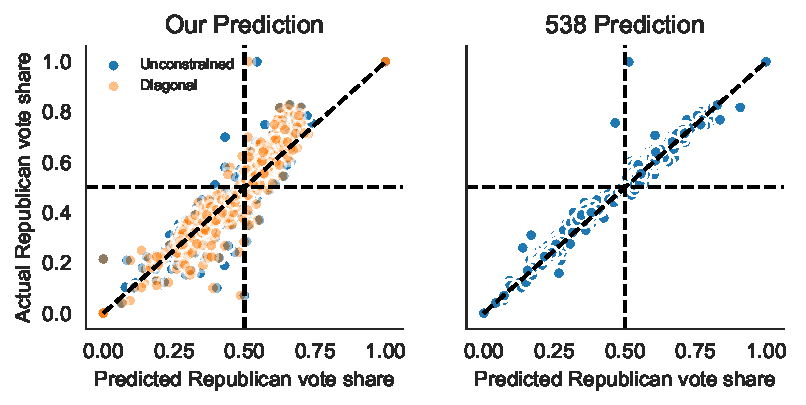
\includegraphics{prediction_quality.pdf}
  \caption{Quality of our prediction compared to that of FiveThirtyEight. }
  \label{fig:quality}
\end{figure}

\begin{table}[tb]
  \caption{Number of correctly called races for each model by winning party of each district, and number of expected seats won by Democrats compared to ground truth.}
  \label{tab:res}
  \vspace{1em}
  \centering
\begin{tabular}{lllll}
\toprule
{} & Total & Diagonal & Unconstrained &  538 \\
Winner                             &       &          &               &      \\
\midrule
Democrat                           &   240 &      216 &           211 &  226 \\
Republican                         &   195 &      190 &           187 &  193 \\
\midrule Expected Democratic Seats &   240 &      230 &           223 &  233 \\
\bottomrule
\end{tabular}

\end{table}



\end{document}
